% https://github.com/MCG-NKU/NSFC-LaTex
% https://www.overleaf.com/read/jydxqkkkskzp
% by Ming-Ming Cheng https://mmcheng.net
% 关于VsCode LaTeX的配置 https://www.cnblogs.com/ourweiguan/p/11785660.html

\documentclass[12pt]{article}


\usepackage[UTF8]{ctex}
\usepackage{nsfc}


%\usepackage{fontspec}
%\usepackage{xcolor}
%\defaultfontfeatures{Ligatures=TeX}




\newcommand{\lyc}[1]{\textcolor[rgb]{0,0.6,0}{LYC: #1}}
\newcommand{\todo}[1]{{\textcolor{red}{\bf [#1]}}}
\newcommand{\myPara}[1]{\paragraph{#1:}}

\graphicspath{{figures/}}


\begin{document}



%%%%%%%%% TITLE

\title{科研与教学陈述}

\maketitle


\begin{center} {李元春} \end{center}


\section{研究概述}

% 本人研究兴趣为软件工程、移动计算和人工智能的交叉领域,尤其关注移动端和云端大数据平台及人工智能软件中的隐私、安全、可靠性等问题,在相关领域顶级会议(如ICSE,FSE,ISSTA,UbiComp,MobiCom,SIGIR等)上发表论文二十余篇,其中包括CCF-A类会议第一作者长文9篇、短文或工具论文2篇。本人主导的工作获得了CCF A类会议UbiComp的最佳论文提名奖,以及领域知名会议IS-EUD的最佳论文奖,相关工具在开源软件平台上被广泛应用。
1991年,著名计算机科学家Mark Weiser提出了普适计算(Ubiquitous Computing)的构想,主张将计算嵌入到环境或日常工具中去,使人能随时随地自然地使用各种计算服务。如今,这一构想已成为现实,以智能手机、智能汽车、机器人等为代表的移动和物联网终端设备迅速发展,在我们日常生活中扮演着越来越重要的角色。同时,随着近年来人工智能技术的飞速进步,将人工智能与普适计算技术结合起来已成为大势所趋。一方面,终端设备上丰富的数据可以为机器学习模型提供养料,另一方面,优秀的模型又可以极大地拓宽和改善终端设备提供的服务。我们正加速进入智能物联(AIoT)时代。

AIoT的可靠性(Reliability)是其长远发展路途中的关键主题之一,其包含两方面的含义,一方面是AIoT系统是否能够保障生态系统中每一方的权利和利益,如个人隐私、知识产权等。另一方面是AIoT提供的服务是否足够健壮和可信,避免产生故障或遭受攻击。
随着用户意识的觉醒、企业对商业利益的考虑、以及各地政府政策的出台,AIoT的可靠性在产业中的重要性越来越凸显。

因此,我主要面向AIoT的可靠性展开研究工作。我的总体研究风格倾向于从真实问题出发,从软件分析和系统设计的角度尝试寻找问题的解决方案。如图~\ref{fig:overview}所示,我的工作面向AIoT生态中流通的三个关键对象,即数据、应用程序和机器学习模型,分别研究数据的隐私与合规、应用的分析与测试、以及模型的健壮性与安全性。


\begin{figure}
    \centering
    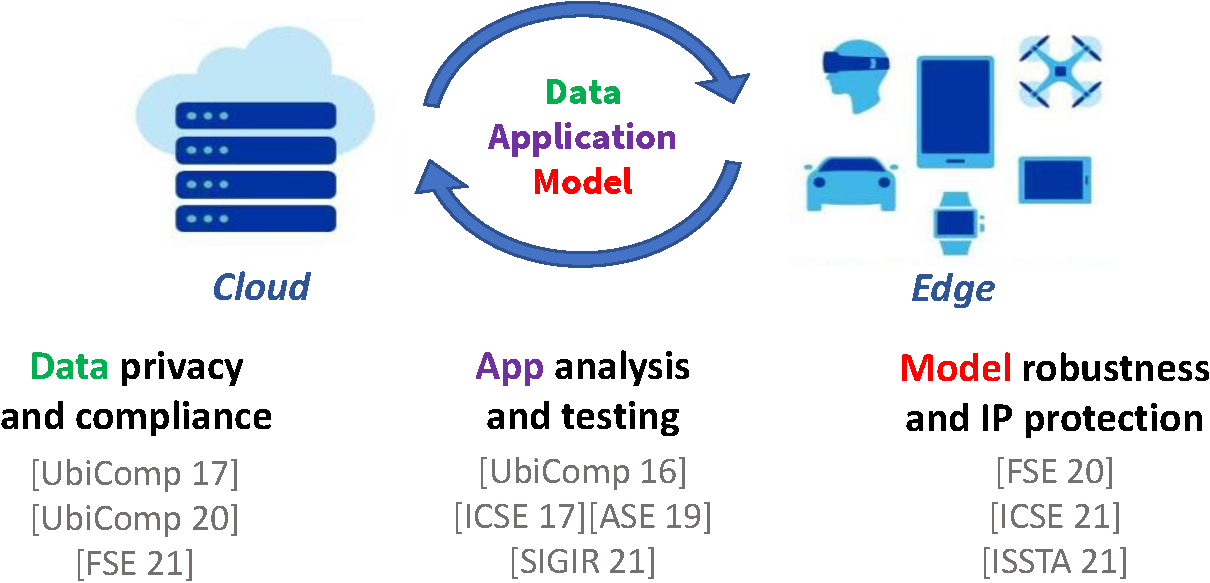
\includegraphics[width=5in]{figures/research_overview.pdf}
    \caption{研究工作概览}
    \label{fig:overview}
\end{figure}

\section{代表性工作}

\subsection{云-端协同数据处理及隐私保护框架}

数据是人工智能技术的重要基石,如何获得大量的、有价值的数据是一个人工智能模型成功的关键。如今无处不在的移动和IoT设备是一个非常重要的数据来源,而如何在收集和处理这些数据的时候尊重用户的隐私,则是每个公司必须要考虑的问题。
我的研究工作是从数据处理框架设计的角度出发,尝试创造一个云端统一、简单易用、保护隐私的用户个人数据处理框架。具有代表性的是PrivacyStreams~\cite{li2017privacystreams}和TaintStream~\cite{yang2021taintstream}系列工作。

首先,我们观察到,云端和终端的数据处理框架是截然不同的。在云端和数据中心中,数据处理往往采用成熟统一的的流式处理框架(如Spark),而在移动系统中,个人数据的组织形式十分异构,处理方式非常碎片化。例如在Android系统中,访问位置、读取通讯录、录音等分别是截然不同的方式,其数据处理操作也很分散随意,难以进行隐私审查。
因此,我们提出了一个全新的移动端流式数据处理框架PrivacyStreams,通过基于大量实证分析的编程接口设计,使移动应用开发者可以用与Spark类似的方式,方便地访问和处理移动端各类个人和传感数据。同时,通过对框架中的编程模型和操作符进行规约设计,我们可以结合静态分析,对程序中使用的隐私数据粒度进行隐私分析。经过由真实开发者参与的用户实验,我们证明了PrivacyStreams可以在一些常见任务上将开发效率提升一倍,并使得开发的程序更加隐私透明。

PrivacyStreams将云端和终端的数据处理方式统一成了基于流的形式。更进一步,我们考虑如何在这种流式数据平台中进行自动的隐私合规约束。这个问题也是目前大部分公司很关心的问题,由于GDPR等规定的施行,很多公司需要耗费大量人工检查各种隐私合规问题,比如数据留存,访问控制,用户退出等等。污点追踪(taint tracking)是一个学术界比较常用的方法,通过修改系统监控敏感数据流动,但在这种大数据情况下,实现起来非常复杂。于是我们提出了一个新的框架TaintStream,通过动态代码翻译的方法实现了轻量级、细粒度的污点追踪,基本的思路是让原始的代码在运行时自动转变成具有相同功能,但会同时传播污点标签的代码。基于这套系统,我们可以高精度、低代价地自动对数据进行各种隐私管理,从而大大降低人工进行隐私合规性检查的成本。

这一系列工作发表在普适计算和软件工程的顶级会议上,在开源社区取得了一定知名度(200+ stars)\cite{privacystreams:code},并受到了国内外媒体的报导。

% 数据的获取和处理是机器学习的关键步骤,尤其是移动端的数据具有很大的利用价值。而同时,由于移动端数据的高度敏感性,以及如今世界各国严格的隐私保护要求(如GDPR等),保护移动用户的隐私也尤为关键。本工作提出一个移动端隐私数据编程框架,在向开发者提供简单易用的流式编程接口的同时,减少代码数据流的碎片化,并进一步通过静态分析获取数据操作的敏感程度。该成果\cite{li2017privacystreams}发表在普适计算领域CCF-A类会议UbiComp 2017中,其对应工具在GitHub获得200多个星标\cite{privacystreams:code},并受多家媒体报道。

\subsection{基于交互界面的应用程序分析与测试}

本人博士期间的研究主要面向移动应用,以软件的图形交互界面为切入点对应用程序的功能和隐私特性进行分析。例如,通过程序静态分析和动态分析相结合的方法提取出应用界面与程序代码间的对应关系,以便于理解和自动判别软件中的隐私数据访问行为是否符合用户认知。同时,通过使用大量软件图形界面进行机器学习,可以自动学习到应用程序的交互模式,从而进一步指导应用程序的自动测试生成和动态分析。代表成果\cite{li2016peruim}发表在普适计算领域CCF-A类会议UbiComp 2016中并获得最佳论文提名奖,其相关联工具DroidBot\cite{li2017droidbot}和Humanoid\cite{li2019humanoid}在开源代码托管平台GitHub获得500多个星标\cite{droidbot:code},为领域内熟知。
 

\subsection{基于软件分析的模型安全保障技术}

程序切片技术是传统程序分析、调试、测试的重要方法之一,旨在从程序代码中提取出与特定关注对象(如变量、API等)相关的子集(切片)。该工作探索了在神经网络中实现程序切片技术的可行性和可能应用。我们提出一种基于正向和反向数据流分析的方法,给定一组输入和输出,可以提取出在模型决策过程中,对预测结果贡献关键作用的神经元子集。该切片技术可以用来分析和解释神经网络决策逻辑,例如可以通过切片模式的差异检测对抗样本、根据神经元的贡献大小对模型进行剪枝等等。工作成果\cite{zhang2020dynamic}发表在软件工程领域CCF-A类会议FSE 2020中。

\textbf{边缘端神经网络模型后门攻击。}
边缘端部署的模型很多被用于安全攸关的场景,例如人脸验证、自动驾驶、安防监控等,因此其安全性和可信性尤为重要。该工作主要关注边缘端模型的后门攻击。与传统基于训练数据投毒或二次训练的后门攻击不同,边缘端部署的模型往往已经经过编译压缩,无法继续训练,同时其输入为物理世界的图片而非可以随意进行像素修改的数字输入。本工作受传统软件中的逆向工程方法启发,提出了一个直接在模型计算图上插入恶意旁路的攻击方法,可以在不需要训练的情况下,向目标模型中插入高效、轻量级的后门逻辑。通过对两万多个真实移动应用的扫描分析,我们成功攻击了52个应用中的模型,其中包括下载量数千万的流行应用和安全攸关的支付、商业、儿童教育类应用。工作成果\cite{li2021deeppayload}发表在软件工程领域CCF-A类会议ICSE 2021中。


\section{未来科研计划}

\subsection{基于移动端分布式机器学习的群体智能研究}
如何理解自然界中的群体智能以及实现人工群体智能是我个人非常感兴趣的研究问题,移动设备丰富的传感能力和逐渐增强的计算能力为群体智能的发展提供了前所未有的机遇。受普适计算领域的众包、群智感知等概念的启发,我希望进一步研究如何让移动个体之间共享知识、共同学习,从而处理更大规模的感知和决策问题,例如如何让家庭和工厂中的智能设备自动协调合作、如何利用泛在的移动设备自动感知城市和环境的状态等等。这其中涉及到系统的搭建、大规模学习节点的性能、容错性,以及节点之间的隐私性等问题亟待解决。

\subsection{软件交互界面的语义理解}
作为之前研究工作的延续,我计划继续以软件交互界面为切入点进行智能软件工程相关的研究。尤其是如今计算机视觉和自然语言处理技术蓬勃发展,为软件交互界面语义理解带来了新的机遇。作为一个多模态的数据类型,对软件交互界面的分析需要同时考虑文本、图像、代码等信息,具有独特的挑战。同时,交互界面的语义理解可以赋能各种新型软件工程任务,例如自动测试、软件无障碍化、机器流程自动化(RPA)等。

\section{教学概述}

我深信教学相长、温故知新的道理,参与教学不仅是身为一个教师的职责,同时也是一个反思和凝练研究工作的过程。

在攻读博士期间,我曾多次作为助教,协助导师参与各项课程的教学,如《计算机系统导论》、《操作系统》、《编译原理》等。我的工作内容包括部分课件的制作、专题的讲授、作业批改和答疑、讨论课的组织等等。这些经历一方面使我熟悉了一门课程背后的运作模式、锻炼了总结和讲授的能力,同时也通过与老师同学的讨论和互动,学到了很多新的知识。

在读期间,我还多次作为The Honeynet Project组织的成员,担任Google Summer of Code开源项目的导师,指导国内外学生参与开源项目。从这些这些经历中,我体会到如何帮助学生指定项目计划,管理项目的进度,从而推进项目的成功。同时,与世界各地同行在开源项目上的合作和交流也让我增长了很多见识。

毕业之后,我在微软亚洲研究院工作期间指导过多个实习生参与科研,其中大部分的实习时间为六个月以上。对于每个实习生,我带领其完成一个研究项目从无到有的全过程,包括如何寻找研究问题、如何制定解决方案、如何进行学术演讲、以及如何撰写学术论文。大部分实习生都在我的指导下完成了一个完整的研究项目,并整理成了论文。在帮助他们成功的同时,我也获得了莫大的成就感。




\section{预计可讲授课程}

\subsection{《智能软件工程》}
卡内基梅隆大学开设有两门与智能软件工程相关的课程,分别是 AI4SE \cite{cmu:ai4se} 和 SE4AI \cite{cmu:se4ai},分别讲解如何用AI技术解决软件工程中的经典问题(如代码分析、需求分析、测试等)和如何用软件分析技术解决AI模型相关的重要问题(例如模型鲁棒性测试和验证、决策过程分析与解释、模型调试等)。我对这两个方向都较为熟悉,可以讲授相关课程。

\subsection{《人工智能的安全、隐私与伦理》}
神经网络的安全隐私及伦理问题是如今热门的研究方向之一,已有很多大学开设了相关课程 \cite{ucb:trustworthy,ucb:fairness}。我在微软亚洲研究院开源课程《人工智能系统》 \cite{microsoft:ai-system}中担任安全与隐私章节的讲师,也对该方向做过调研和整理,可以讲授相关课程。

\subsection{《计算机系统》、《编译原理》、《软件工程》}
我在本科学习期间就对这些课程就有着浓厚的兴趣,在取得了优异的成绩的同时,直接促使我选择了相关方向的实验室和导师展开了科研工作。博士在读期间,又多次担任这些基础课程的助教,进一步加深了对相关课程内容的理解,并熟悉了课程背后的教案准备、作业批改、试题设计等内容。这些基础课程是历久弥新的,对我的研究工作也有温故知新的作用,因此我也可以讲授这些基础课程。


{
\bibliographystyle{ieee_fullname}
\bibliography{lyc}
}


\end{document}
